%Appendix -- January 2015
\appendix
\renewcommand{\thechapter}{B}
\renewcommand{\chaptername}{Appendix}

\chapter{New apparatus}
\label{app:new_apparatus}

As mentioned in the main text, the construction of a new apparatus for producing BECs of $\Rb87$ and $^{39}$K is underway. The design of the apparatus is intended to be a bug fix version of the RbChip~\cite{AbyThesis} lab at NIST. The new apparatus does not have a Zeeman slower and instead will use magnetic transport coils to move atoms from a MOT cell to the main science cell. 

This Appendix describes some aspects of the design and construction of the new apparatus where I was involved. Disclaimer: none of this things have been tested yet so we don't know yet if it will all work horribly. I have listed all relevant part numbers in case replacements are needed. 

\section{Water cooling}

The lack of a Zeeman slower in the apparatus greatly simplifies the water cooling system compared to that of RbLi. Since we don't anticipate to have any coils with high flow impedance we expect that the pressure from a recirculating chiller will be enough to provide water cooling to the transistor banks and the magnetic transport coils. 

Our choice of chiller was the \noted{TF1LN400-LN} $\unit[1.4]{kW}$ recirculating chiller from \noted{Thermo Fisher Scientific}. The water is filtered both at the output and the return with a high-impedance filter with a cellulose cartridge (filter: Mcmaster \noted{4422K3}, cartridge: McMater \noted{7191K11}). A breakout manifold divides the chilled water into 5 different lines, each one with a flow meter (\noted{Proteus Industries 0101C110}) that can be used to interlock the current of water cooled applications to the flow of water. Based on previous experiences with plumbing (see Appendix~\ref{app:RbLi}) I highly encourage replacing the filters at least once a year and to use a solution of $10\%$ corrosion inhibitor (e.g. OptiShield Plus) and distilled water as a coolant. 

\begin{figure*}[htb]
\begin{center}
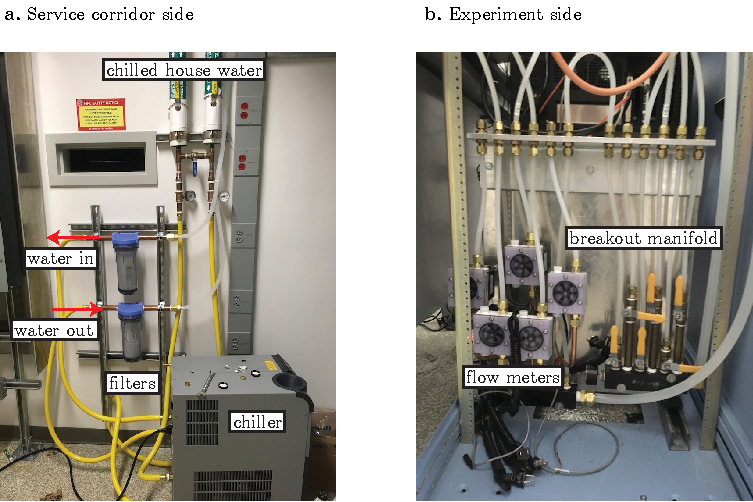
\includegraphics[]{Figures/AppendixB/plumbing.pdf}
\caption[Water cooling]{Water cooling}
\label{fig:plumbing}
\end{center}
\end{figure*}

\section{Electrical installation}
We have two \noted{Agilent 6690A} ($\unit[440]{A}$ at $\unit[15]{V}$ max. current) to provide all the necessary currents. The power supplies are located in the service corridor and are connected to three copper bars corresponding to $\unit[\pm 15]{V}$ and ground using welding cable (McMaster \noted{7818A17}) that is laid on cable trays (McMaster \noted{30065T11} e.g.). The cables are arranged in the pattern shown in Figure xxx so that the magnetic field produced by them is closer to a magnetic quadrupole which decays faster than the field of a magnetic dipole. We are not planing to use commercial bipolar power supplies in this lab (see Appendix~\ref{app:RbLi}) and instead we will be using a MOSFET based homemade device that will draw current from the $\unit[\pm15]{V}$ rails. 

\begin{figure*}[htb]
\begin{center}
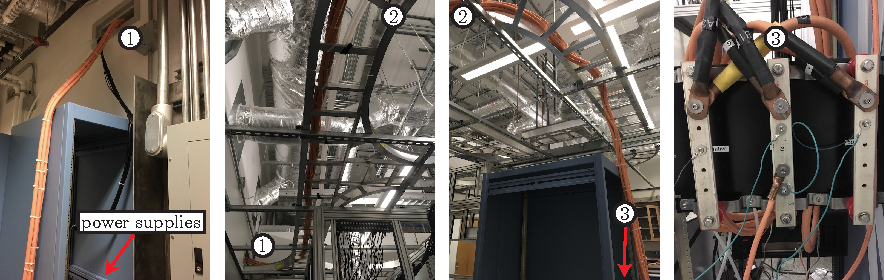
\includegraphics[]{Figures/AppendixB/electric.pdf}
\caption[Electrical installation]{A roller coaster ride, from the power supplies in the service corridor to three copper bars that distribute the power.}
\label{fig:plumbing}
\end{center}
\end{figure*}

\section{Coil winding}
All the coils in the apparatus including magnetic transport, bias and gradient cancellation have been wound using \noted{Laminax} ribbon wire from \noted{Bridgeport Magnetics}. We followed the the coil fabrication process described in~\cite{AbyThesis} which involves first winding a fixed number of turns around a prefabricated form with a particular geometry. The coils were then covered with a machinable epoxy (\noted{Stycast 1266}) to fill in any air gaps. A lesson we learned while doing this is that only room temperature epoxy should be mixed. We keep the epoxy in a fridge to extend its lifetime but if it is cold some tiny drops of water will condense in it as it is being mixed and it will not properly be cured. To minimize the air bubbles we placed the coils with epoxy on a vacuum bell and we pumped the air out using an electric vacuum pump (\noted{McMaster 4396K21}). After the epoxy has cured (overnight if it is left at room temperature or less if it is left at higher temperature) the coils are ready for lathing to remove all excess epoxy and kapton tape up to the surface of the copper. After some trial and error (and lots of frustration) we found that using a diamond tip cutter (\noted{McMaster 3316A32}) and spinning the lathe not faster than $\unit[150]{rpm}$ the best results. Using a cutter that is not sharp enough or cutting too aggressively close to the soft copper results in deformed rather. In the past when coils were fabricated at NIST a lathing form was used to mount the coils on the lathe. The machinist at UMD considered this was not safe enough so I instead mounted the coils using a 6 jaw chuck as shown in Figure~\ref{fig:coil_winding}a. than cut traces that merge into each other causing unwanted shorts. For anyone making coils in the future: it is sort of an art to get it right and screwing up many coils is part of learning the art. 

\begin{figure*}[htb]
\begin{center}
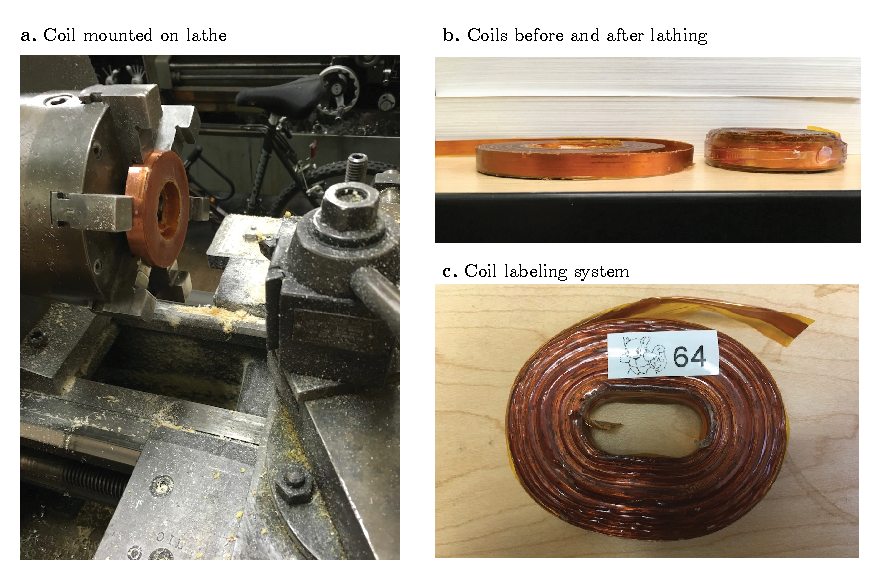
\includegraphics[]{Figures/AppendixB/coil_winding.pdf}
\caption[Electrical installation]{A roller coaster ride, from the power supplies in the service corridor to three copper bars that distribute the power.}
\label{fig:coil_winding}
\end{center}
\end{figure*}

\section{Rb source and `oven'}
The Rb source consists of a $1.33"$ CF flanged bellow (\noted{Kurt J. Lesker} \noted{MH-CF-A03}) with a Rb ampule . The bellow is housed in a cold `oven' which is designed to keep the source at a temperature $\approx \unit[1]{C}$ to keep the vapor pressure low. The oven is made of hollow aluminum cylinder with a slit on one side with tapped holes so that $1/4-20$ screws can be used to fix the oven to the source. The bottom of the oven attaches to the cold end of a TEC that provides the cooling. The hot side of the TEC is attached to a heat sink made of a hollow brass piece with tapped holes for $1/4"$ NPT pipes are used to provide water cooling. The left panel of Figure xxx shows CAD drawings of the oven both of this parts and the right panel shows the actual parts mounted on a test bench. The Rb source will be connected to the MOT glass cell; the plan is to use light induced atomic desorption (LIAD)\cite{anderson_loading_2001} to increase the Rb vapor pressure for MOT loading using non-thermal means. 

Our initial hope was to control the temperature using a linear temperature controller designed at the JQI (the design is available at the \href{https://github.com/JQIamo/Linear-Temperature-Controller}{JQI GitHub}) interfaced to the lab computer andLabscript using a serial to ethernet adapter (\noted{WIZnet WIZ107SR}). Unfortunately this project is not completed to this date.  

\begin{figure*}[htb]
\begin{center}
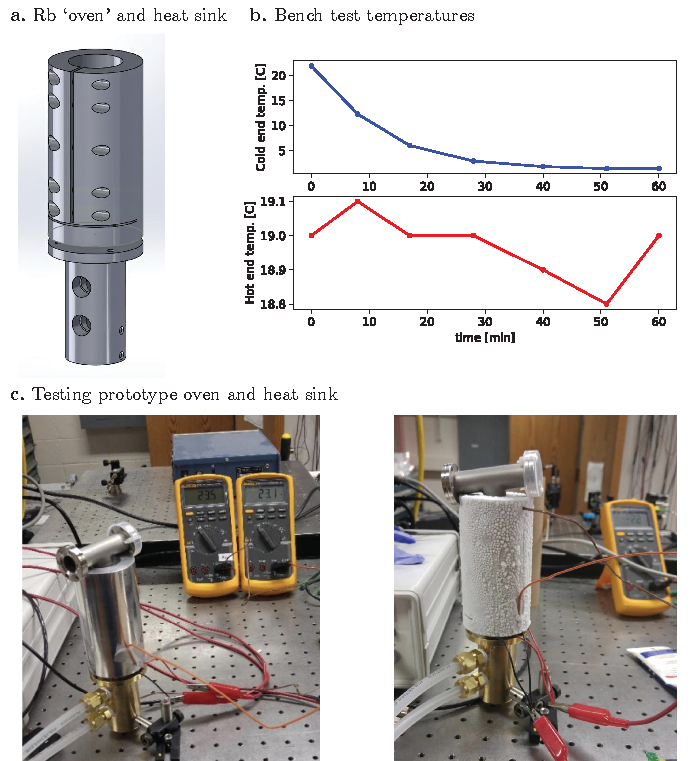
\includegraphics[]{Figures/AppendixB/rb_source.pdf}
\caption[Rubidium oven assembly]{Rubidium oven assembly}
\label{fig:rb_source}
\end{center}
\end{figure*}

\section{Table enclosures}
The enclosures of the optical tables are made of $\noted{Alumalite}$ from \noted{Laminators Inc.} mounted on frames made out of aluminum extrusions from \noted{80/20} and sliding tracks (\noted{2220} and \noted{2210}). Alumalite is a sandwich of a corrugated corrugated polypropylen material in between two thin sheets of aluminum. We chose this material because it is strong and lightweight. Its laser safety properties remain to be tested but we anticipate it is better than the acrylic panels at the RbLi lab. The initial frames were designed and built mostly by former graduate student Daniel Campbell and later finished and modified by former undergraduate student Eliot Fenton and me.  

To the new and future members of the lab: I sincerely hope the things I designed and built don't cause you much pain!

